% Synchronized to r43697
\subsection{OPT\_IGMPPROXY - Internet Group Management Protocol Proxy)}
\configlabel{OPT\_IGMPPROXY}{OPTIGMPPROXY}

The German Telekom AG offers VDSL25/50 for some years now (Bandwidth: 25/50 MBit/s)
in so-called Entertain packages. This enables to watch TV over the Internet (IPTV).

IPTV is provided via Multicast, from one source to a (closed) group. The network protocol
needed to organize Multicast groups is called IGMP (Internet Group Management Protocol).
IGMP (\altlink{http://en.wikipedia.org/wiki/IGMP}) provides the ability to dynamically
manage Multicast groups. The administration is not done in the transmitting station but
by the routers to which recipients of a multicast group are connected directly. IGMP
provides functions by which a station notifies a router that it wants to receive
multicast IP packets of a particular multicast group.

The provided Speedport routers (W700V/W701V/W722 by the time of writing) support IGMP.
Those who want to use fli4l for IPTV instead of those Speedport routers, need an IGMP-Proxy
(\altlink{http://sourceforge.net/projects/igmpproxy/}) on the fli4l.
OPT\_IGMPPROXY is a IGMP-Proxy for fli4l.

This documentation for the package OPT\_IGMP describes the configuration of fli4l
to use VDSL and IPTV with the supplied set-top box (STB) X300T/X301T or MR-303 behind
a fli4l router. In this description, the installation of IPTV via an additional network
card is assumed.


\subsubsection{Precondition}

The German Telekom introduced VDSL as a VLAN. In the introductory phase only one VLAN tag (ID7)
was used for all traffic. After that they switched to two VLAN tags (ID7, ID8). The Internet traffic
remains on ID7 and the new ID8 is used exclusively for IPTV multicast traffic. The conversion
of VDSL (two VLAN tags ID7/ID8) is largely completed by the current state.

Hardware (besides Set-Top-Boxes and VDSL-Modem):
\begin{itemize}
   \item{Hardware for fli4l: For VDSL 25/50 more than an i486. In case of sound or image distortions
   it may be that the hardware used has too little power.}
   \item{High-End network interface cards (Examples: 3Com, Intel Pro100). Realtek chipsets are not recommended.}
\end{itemize}

Software:
\begin{itemize}
   \item{Package: advanced\_networking}
   \item{Package: dhcp\_client (for the use of ID8)}
\end{itemize}

The following describes adapting the config files base.txt, dsl.txt, advanced\_networking.txt, dhcp\_client.txt, dns\_dhcp.txt.

\subsubsection{Hardware Setup}

The recommendation to connect the IPTV SetTopBox without further network elements directly
to the router also applies to fli4l. If network nodes like hubs, switches, bridges, gateways,
or routers have to be placed between the IPTV box and fli4l, these should be multicast-enabled
to avoid problems.

Home networks usually do not use switches that separate virtual networks (VLAN) from each
other in order to disencumber remaining traffic (ID7) from IPTV multicast traffic (ID8).
This is why a separate NIC (Network Interface Card = LAN or Ethernet card) is used to
connect the set-top box (STB) directly to fli4l to avoid all problems due to heavy traffic.
Those preferring the single NIC method (not described here) should know what to do on their own.

The easiest way to use an IPTV STB hence is to install an additional NIC to fli4l's hardware.

Find a diagram below how to migrate fli4l from standard to a third NIC:

\begin{itemize}
   \item{Standard configuration:
         \begin{itemize}
            \item{eth0 is used as the NIC for internal home/office LAN in base.txt}
            \item{eht1 is the DSL interface mentioned in dsl.txt}
         \end{itemize}
         \begin{figure}[ht!]
         \centering
         \fontfamily{phv}\selectfont VDSL modem~~~~~fli4l router~~~~~~~~~~~~~~~~\\
         
\includegraphics[]{image001}\\
         ~~~~~~~~~~~~~~~~~~~~~~~~~~~~~~~~~~~~~~~~~~~~LAN interface
         \caption{fli4l in a standard configuration}
         \label{fig:standardconfig}
         \end{figure}
      }
   \item{Advanced configuration with an additional IPTV NIC:
         \begin{itemize}
            \item{After installation of an additional NIC eth2 has to be inserted in base.txt.}
         \end{itemize}
         \begin{figure}[ht!]
         \centering
         \fontfamily{phv}\selectfont ~~~~~~~VDSL modem~~~~~fli4l router~~~~~IPTV-STB interface\\
         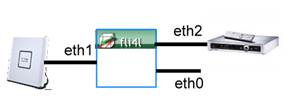
\includegraphics[]{image002}\\
         ~~~~~~~~~~~~~~~~~~~~~~~~~~~~~~~~~~~~~~~~~~~~LAN interface
         \caption{fli4l in an IPTV configuration}
         \label{fig:iptvconfig}
         \end{figure}
      }
\end{itemize}


\subsubsection{VLAN Configuration}

First of all: OPT\_IGMP is not depending on VLAN. VLAN is needed for Deutsche Telekom VDSL and hence
should be supported by the router. Whether VLAN is required for other providers (Arcor, Alice, a.s.o. ..)
is beyond our knowledge at the moment.

To get VDSL25/50 as provided by T-Home up and running, the NIC to the VDSL modem necessarily has to be
configured as a VLAN interface.

\vspace{3mm}
\emph{A note for those using only 'normal DSL', ie ADSL, ADSL2, ADSL2+: VLAN is only needed by VDSL,
      but not for 'normal DSL' - the VLAN configuration will not work in this case.}
\vspace{3mm}

If two VLAN tags are used (see above) traffic is split as follows:

\begin{itemize}
   \item{VLAN ID7: Internet traffic}
   \item{VLAN ID8: IPTV Multicast traffic}
\end{itemize}

This way Internet traffic is independent from IPTV traffic. The main difference
is that VLAN ID7 needs a PPPoE dial-in. VLAN ID8 is provided via a DHCP server
without dial-in. In this architecure there is no forced disconnect after 24
hours any more.\\

The following configuration is needed for VLAN (hardware setup of NICs as
described above):\\

\noindent \textbf{advanced\_networking.txt}

\begin{example}
\begin{verbatim}
VLAN_DEV_N='2'
VLAN_DEV_1_DEV='eth1’     # interface of VDSL-Modem; example: eth1
                          # in our example 'eth1' connects to the VDSL modem
VLAN_DEV_1_VID='7         # ID7 to support VLAN for internet
VLAN_DEV_2_DEV='eth1’     # interface of VDSL modem; example: eth1
VLAN_DEV_2_VID='8’        # ID8 to support VLAN for IPTV
\end{verbatim}
\end{example}

\noindent The virtual NIC eth1.7 has to be inserted into the DSL configuration:\\

\noindent \textbf{dsl.txt}

\begin{example}
\begin{verbatim}
PPPOE_ETH='eth1.7'        # eth<number of the card connecting the vdsl modem>.7'
                          # i.e. 'eth1.7'
\end{verbatim}
\end{example}

\noindent The virtual NIC eth1.8 needs a dhcp\_client, because VLAN
ID8 is provided by a DHCP server without dial-in.\\

\noindent \textbf{dhcp\_client}

\begin{example}
\begin{verbatim}
OPT_DHCP_CLIENT='yes'
DHCP_CLIENT_TYPE='dhcpcd'
DHCP_CLIENT_INTERFACES='IP_NET_3_DEV' # listen on interface eth1.8
DHCP_CLIENT_USEPEERDNS='no'
DHCP_CLIENT_HOSTNAME=''
\end{verbatim}
\end{example}

As of fli4l V3.3 the interface can only defined by the value of \texttt{IP\_NET\_x\_DEV}
defined for the interface in base.txt, here: \texttt{IP\_NET\_3\_DEV}. Specifying
\texttt{eth1.8} is not possible anymore.\\

\noindent Optional:\\
If the NIC in use has problems with the MTU size it can be adapted with the
parameter DEV\_MTU. Intel Pro/100 (e100) and a 3-Com card worked well during
tests without changes, but a 3Com '3c59x' was reported to need a MTU of 1496.

\begin{example}
\begin{verbatim}
DEV_MTU_1=''              # Adjust MTU size of NIC on VDSL-Modem
                          # Example: DEV_MTU_1='eth1 1496'
\end{verbatim}
\end{example}

The config files base.txt and dns\_dhcp.txt have to be changed as described
in the next chapter.\\

\subsubsection{Configuration Of An Additional NIC For IPTV}

In base.txt and dns\_dhcp.txt the configuration has to be changed for
VLAN and for the second NIC.\\

\noindent Insert the second NIC for IPTV:\\

\begin{example}
\begin{verbatim}
NET_DRV_N='2'
NET_DRV_1='via-rhine'     # 1. NIC interface for LAN
NET_DRV_2='3c59x'         # 2. NIC – here 3Com for IPTV SetTopBox
\end{verbatim}
\end{example}

Now the address range for the second NIC has to be set. We will use
192.168.2.0/24 for the LAN and 192.168.3.0/24 for the second NIC.
Entries for the virtual NICs eth1.7 and eth1.8 are needed in addition:\\

\begin{example}
\begin{verbatim}
IP_NET_N='4'
IP_NET_1='192.168.2.1/24'           # home/office LAN
IP_NET_1_DEV='eth0'
IP_NET_2='192.168.3.1/24'           # iptv LAN
IP_NET_2_DEV='eth2'
IP_NET_3='dhcp'                     # dhcp client - IP via dhclient
IP_NET_3_DEV='eth1.8'
IP_NET_3_MAC='00:40:63:da:cf:32'    # new MAC (not the MAC of eth1)
IP_NET_4='dhcp'                     # eth1.7 connecting to the modem
IP_NET_4_DEV='eth1.7'
IP_NET_4_MAC='00:40:63:da:cf:33'    # new MAC (not the MAC of eth1)
\end{verbatim}
\end{example}

It is important to change the MAC addresses for eth1.7 and eth1.8 to
be different from eth1's one, otherwise - depending on the VDSL net
disturbances can occur after forced disconnection.

For the new NIC Internet access must be possible, just as
for the first NIC. These additional settings are necessary:\\

\begin{example}
\begin{verbatim}
PF_INPUT_1='IP_NET_1 ACCEPT'
PF_INPUT_2='IP_NET_2 ACCEPT'
PF_INPUT_3='any 224.0.0.0/4 ACCEPT'
[...]
PF_FORWARD_3='any 224.0.0.0/4 ACCEPT'
PF_FORWARD_5='IP_NET_1 ACCEPT'
PF_FORWARD_6='IP_NET_2 ACCEPT'
[...]
PF_POSTROUTING_1='IP_NET_1 MASQUERADE'
PF_POSTROUTING_2='IP_NET_2 MASQUERADE'
\end{verbatim}
\end{example}

For working dynamic DHCP addressing at the new IPTV NIC and to access
the set-top box by its name, the following settings in dns\_dhcp.txt are
required:\\

\begin{example}
\begin{verbatim}
HOST_10_NAME='igmp'
HOST_10_IP4='192.168.3.1'
HOST_11_NAME='iptv'
HOST_11_IP4='192.168.3.4'
HOST_11_MAC='00:D0:E0:93:49:34'         # MAC Adr T-Home X300T
[...]
DHCP_RANGE_2_NET='IP_NET_2'
DNSDHCP_RANGE_2_START='192.168.3.10'
DNSDHCP_RANGE_2_END='192.168.3.20'
DNSDHCP_RANGE_2_DNS_SERVER1=''
DNSDHCP_RANGE_2_DNS_SERVER2=''
DNSDHCP_RANGE_2_NTP_SERVER=''
DNSDHCP_RANGE_2_GATEWAY=''
\end{verbatim}
\end{example}

After configuring the new NIC it is suggested to connect it to a PC to see if
Internet access is possible over it. In case of success the new second
NIC should be configured correctly.

\subsubsection{IGMP Functions}

When booting the fli4l router the parameters of the config file proxy.txt
are written to the file /etc/igmpproxy.conf, which is read when starting
igmpproxy.

In contrast to earlier versions of opt\_igmp the IGMP proxy is started at
boot and then runs as long as a physical Internet connection is available.
The IGMP proxy is not affected by a forced disconnetion after 24 hour or
manual connect or disconnect of Internet traffic.

\subsubsection{IGMP Configuration}

\begin{description}

\config{OPT\_IGMPPROXY}{OPT\_IGMPPROXY}{}

\var{'yes'} activates the IGMP proxy package while \var{'no'}
deactivates it completely.

\config{IGMPPROXY\_DEBUG}{IGMPPROXY\_DEBUG}{IGMPPROXYDEBUG}

By specifying \var{'yes'} here messages of the IGMP proxy are sent to syslog.

\config{IGMPPROXY\_DEBUG2}{IGMPPROXY\_DEBUG2}{IGMPPROXYDEBUG2}

By specifying \var{'yes'} here the log level of the IGMP proxy may be increased.

\config{IGMPPROXY\_QUICKLEAVE\_ON}{IGMPPROXY\_QUICKLEAVE\_ON}{
IGMPPROXYQUICKLEAVEON}

With Quickleave the load in the upstream link can be lowered. If the
parameter is enabled by \var{'yes'}, this will cause that the Multicast
is canceled faster after a channel change and so the downstream load
is lowered by the IGMP proxy behaving like a receiver.

If two STBs exist and show the same channel, it may happen  (with Quickleave
enabled) that the program is interrupted on one box if
switched on the second. When using only one STB Quickleave may safely
be enabled.

\begin{example}
\begin{verbatim}
IGMPPROXY_QUICKLEAVE_ON='yes'      # activate Quickleave mode
                                   # yes or no; Default: yes
\end{verbatim}
\end{example}

\config{IGMPPROXY\_UPLOAD\_DEV}{IGMPPROXY\_UPLOAD\_DEV}{IGMPPROXYUPLOADDEV}

For IPTV operation IGMP proxy requires an upstream and a downstream interface.
The upstream interface is the interface of the NIC attached to the VDSL modem.
This usually should always remain the same.

With the transfer of IPTV to ID8 eth1.8 instead of ppp0 has to be entered
in the configuration file.

\begin{example}
\begin{verbatim}
IGMPPROXY_UPLOAD_DEV='eth1.8'      # Upstream interface; Default: ppp0
                                   # eth1.8 for T-Home/VDSL with id7/id8
\end{verbatim}
\end{example}

\config{IGMPPROXY\_DOWNLOAD\_DEV}{IGMPPROXY\_DOWNLOAD\_DEV}{IGMPPROXYDOWNLOADDEV
}

The interface of the downstream (NIC for IPTV set-top box) is set here
dependent on the hardware configuration. For fli4l with second NIC eth2
is the interface for the set-top box.

\begin{example}
\begin{verbatim}
IGMPPROXY_DOWNLOAD_DEV='eth2'      # Downstream interface
\end{verbatim}
\end{example}

\config{IGMPPROXY\_ALT\_N}{IGMPPROXY\_ALT\_N}{IGMPPROXYALTN}

This parameter specifies the number of address ranges for Multicast streams.

\config{IGMPPROXY\_ALT\_x\_NET}{IGMPPROXY\_ALT\_x\_NET}{IGMPPROXYALTxNET}

By the parameter IGMPPROXY\_ALT\_NET address ranges for Multicast traffic
originating outside of the LAN are defined as well as the local address range
that connects to the STB.

\begin{example}
\begin{verbatim}
IGMPPROXY_ALT_N='3'                        # Number of Multicast sources
IGMPPROXY_ALT_1_NET='239.35.0.0/16'        # IPTV streams - always needed
IGMPPROXY_ALT_2_NET='217.0.119.0/24'       # needed for T-Home
IGMPPROXY_ALT_3_NET='193.158.34.0/23'      # needed for T-Home
                                           # before May 2013 '193.158.35.0/24'
# IGMPPROXY_ALT_4_NET='192.168.3.0/24'     # Address range IPTV SetTop-Box/not
                                           # needed anymore
\end{verbatim}
\end{example}

\config{IGMPPROXY\_WLIST\_N}{IGMPPROXY\_WLIST\_N}{IGMPPROXYWLISTN}

With this parameter the number of whitelists for IGMP reports is
determined.

\config{IGMPPROXY\_WLIST\_x\_NET}{IGMPPROXY\_WLIST\_x\_NET}{IGMPPROXYWLISTxNET}:\newline

Using IGMPv3 all addresses may be summarized in one report which in turn will be
ignored completely. This leads to a complete shutdown of all Multicast traffic by the
IGMP Querier assuming that it is not needed anymore. To avoid this, configuration of
whitelists is used. Only Multicast goups in this list will be requested on the WAN side.

\begin{example}
\begin{verbatim}
IGMPPROXY_WLIST_N='1'                          # Number of Multicast sources
IGMPPROXY_WLIST_1_NET='239.35.0.0/16'         # IPTV streams - always needed
                                               # see above
\end{verbatim}
\end{example}

\end{description}

\subsubsection{Changes In Other Config Files}

As of revision 32955 it is not necessary to adapt the firewall rules for
IGMP Proxy and Multicast streams if the standard rules are activated in
base.txt (\var{PF\_INPUT\_ACCEPT\_DEF='yes'} and \var{PF\_FORWARD\_ACCEPT\_DEF='yes'}).
The start script will automatically add these rules if \var{OPT\_IGMPPROXY='yes'} is set.

There will be two rules added to the INPUT chain to let the IGMP Proxy
receive incoming messages:

\begin{example}
\begin{verbatim}
Chain INPUT (policy DROP 0 packets, 0 bytes)
 pkts bytes target   prot opt in   out   source         destination
 [...]
    0     0 ACCEPT   all  --  *    *     0.0.0.0/0      224.0.0.1     \
    /* automatically added for IGMP Proxy */

    0     0 ACCEPT   all  --  *    *     0.0.0.0/0      224.0.0.22    \
    /* automatically added for IGMP Proxy */
 [...]
\end{verbatim}
\end{example}

Another rule will be added to the FORWARD chain that enables forwarding of
incoming Multicast streams to the media receiver.

\begin{example}
\begin{verbatim}
Chain FORWARD (policy DROP 0 packets, 0 bytes)
 pkts bytes target   prot opt in   out   source         destination
 [...]
    0     0 ACCEPT   all  --  *    *     0.0.0.0/0      239.35.0.0/16  \
    /* automatically added for IPTV streams */
 [..]
\end{verbatim}
\end{example}

If the standard rules are not activated at least the following rules have to be added:

\begin{example}
\begin{verbatim}
PF_INPUT_x='any 224.0.0.1/32 ACCEPT'
PF_INPUT_x='any 224.0.0.22/32 ACCEPT'
[...]
PF_FORWARD_x='any 239.35.0.0/16 ACCEPT'
\end{verbatim}
\end{example}

\achtung{Hint: Despite to earlier versions of the documentation the rules were
   restricted to the nets really needed. If IPTV does not work as exepected
   feel free to provide additional information concerning the nets used.}

\achtung{Important!
By the end of May 2013 the Telekom introduced new classless routes for Entertain
(\altlink{http://www.onlinekosten.de/forum/showthread.php?t=116415&page=38}).
This seems to be caused by the use of more than 256 stations resp. addresses.
The DHCP server now transfers routes not contained in the subnet used before.
As long as the Telekom does not change its iptv-server-subnet (193.158.34.0/23)
a static route may be defined for the vlan8 interface to adapt these changes,
otherwise Multicast would not work anymore.}

Solution: specify an additional route in base.txt.

\begin{example}
\begin{verbatim}
IP_ROUTE_N='1'
IP_ROUTE_1='193.158.34.0/23 eth1.8'
\end{verbatim}
\end{example}
